\documentclass[10pt,a4paper,twocolumn]{article}

\usepackage[margin=1.5cm]{geometry}
\usepackage{graphicx}
\usepackage{booktabs}
\usepackage{microtype}
\usepackage{url}
\usepackage[font=small,labelfont=bf,skip=3pt]{caption}
\usepackage{times}

\graphicspath{{../results/robustness/}{../results/failures/}{../results/clean/}}

\setlength{\parskip}{0pt}
\setlength{\columnsep}{0.6cm}
\setlength{\textfloatsep}{8pt}
\setlength{\floatsep}{8pt}
\setlength{\intextsep}{8pt}

\title{\vspace{-1.3cm}\textbf{Fine-Tuning Helps Against Blur and Hurts Against Noise:\\
Transfer Strategies for Plant Disease Recognition under Field Capture}\vspace{-0.25cm}}

\author{\small Egor Savchenko \quad Zamir Safin \quad Ilia Ponomarev \quad Vadim Poponnikov\\[2pt]
\small Innopolis University --- Computer Vision 2026 --- Project P02\vspace{-0.35cm}}

\date{}

\begin{document}
\maketitle

\section{Problem and question}

PlantVillage is captured in a laboratory: one detached leaf, uniform background, even illumination.
A pretrained ResNet-50 saturates on it, so the interesting question is not whether transfer learning
works but which transfer strategy survives leaving the laboratory. We ask: \emph{does full
fine-tuning of an ImageNet-pretrained ResNet-50 retain its advantage over frozen-backbone linear
probing when leaf images are degraded by realistic robotic field-capture artifacts?} The controlled
variable is which parameters receive gradients; architecture, data, schedule and seed are fixed. We
also report a learning-rate sensitivity study and an analysis of which disease pairs are confused.

\section{Dataset}

PlantVillage (Kaggle mirror), 38 classes over 14 crops. The distribution ships \texttt{train} and
\texttt{val}; we build the test set by \emph{moving} 5\,\% of each training class into \texttt{test}
with seed 42, so no image can appear in two splits, giving 41\,275 / 10\,861 / 2\,169 images.
Images are resized to $224\times224$ and normalised with ImageNet statistics; training adds flips
and rotation up to $15^{\circ}$. Model selection uses validation macro F1 only, and the test split
is read once per run.

\section{Method}

Both conditions start from the same \texttt{ResNet50\_Weights.DEFAULT} checkpoint with the classifier
replaced by a 38-way linear layer. The \textbf{baseline} freezes the backbone and trains only the
classifier (77\,862 of 23\,585\,894 parameters), i.e.\ a linear probe on fixed ImageNet features; the
\textbf{second condition} fine-tunes all 23\,585\,894. Shared settings: AdamW, learning rate
$10^{-4}$, weight decay $10^{-4}$, batch size 64, mixed precision,
\texttt{ReduceLROnPlateau} on validation macro F1, early stopping with patience 5, seed 42.

\textbf{Capture degradation.} To leave the laboratory without changing the label space, we model an
autonomous field phenotyping robot with three independent artifacts, applied to the test images in
capture space at three severities, with a per-image seed derived from the file path:
(i) \emph{motion blur}, a line kernel of 5/11/19\,px at a random angle, for imaging while moving;
(ii) \emph{low light with sensor noise}, where the image is darkened by $0.50/0.30/0.18$, Poisson
shot noise and Gaussian read noise are applied at that signal level, and the result is scaled back
up --- this reproduces a camera raising gain, so mean brightness is restored while
signal-to-noise ratio is not; and (iii) \emph{JPEG compression} at quality 30/15/8, for on-board
compression before radio transmission. The three act through different channels --- optical,
photometric and codec --- so their effects are independent. Neither model is retrained: both are
evaluated on all ten conditions.

\section{Results}

\begin{table}[t]
\centering
\caption{Clean test set (2\,169 images) and training cost.}
\label{tab:clean}
\small
\begin{tabular}{lrr}
\toprule
& \textbf{Frozen} & \textbf{Fine-tuned} \\
\midrule
Trainable parameters & 77\,862 & 23\,585\,894 \\
Epochs to early stop & 47 & 16 \\
Training time (min) & 14.7 & 9.9 \\
\midrule
Accuracy & 0.9696 & \textbf{0.9986} \\
Macro F1 & 0.9664 & \textbf{0.9976} \\
Errors & 66 & \textbf{3} \\
Mean confidence when wrong & 0.531 & 0.859 \\
\bottomrule
\end{tabular}
\end{table}

\begin{table}[t]
\centering
\caption{Accuracy and macro F1 under simulated robotic capture.
Bold marks the better model per row.}
\label{tab:robust}
\footnotesize
\begin{tabular}{llcccc}
\toprule
& & \multicolumn{2}{c}{\textbf{Frozen}} & \multicolumn{2}{c}{\textbf{Fine-tuned}} \\
\cmidrule(lr){3-4}\cmidrule(lr){5-6}
\textbf{Artifact} & \textbf{S} & Acc. & F1 & Acc. & F1 \\
\midrule
Clean & 0 & .970 & .966 & \textbf{.999} & \textbf{.998} \\
\midrule
Motion blur & 1 & .849 & .835 & \textbf{.982} & \textbf{.977} \\
            & 2 & .621 & .557 & \textbf{.853} & \textbf{.802} \\
            & 3 & .463 & .354 & \textbf{.585} & \textbf{.464} \\
\midrule
Low light   & 1 & .866 & .829 & \textbf{.876} & \textbf{.880} \\
+ noise     & 2 & \textbf{.710} & \textbf{.630} & .550 & .492 \\
            & 3 & \textbf{.312} & \textbf{.229} & .138 & .085 \\
\midrule
JPEG        & 1 & .929 & .916 & \textbf{.995} & \textbf{.993} \\
            & 2 & .828 & .794 & \textbf{.948} & \textbf{.941} \\
            & 3 & .654 & .590 & \textbf{.765} & \textbf{.715} \\
\bottomrule
\end{tabular}
\end{table}

\begin{figure*}[t]
\centering
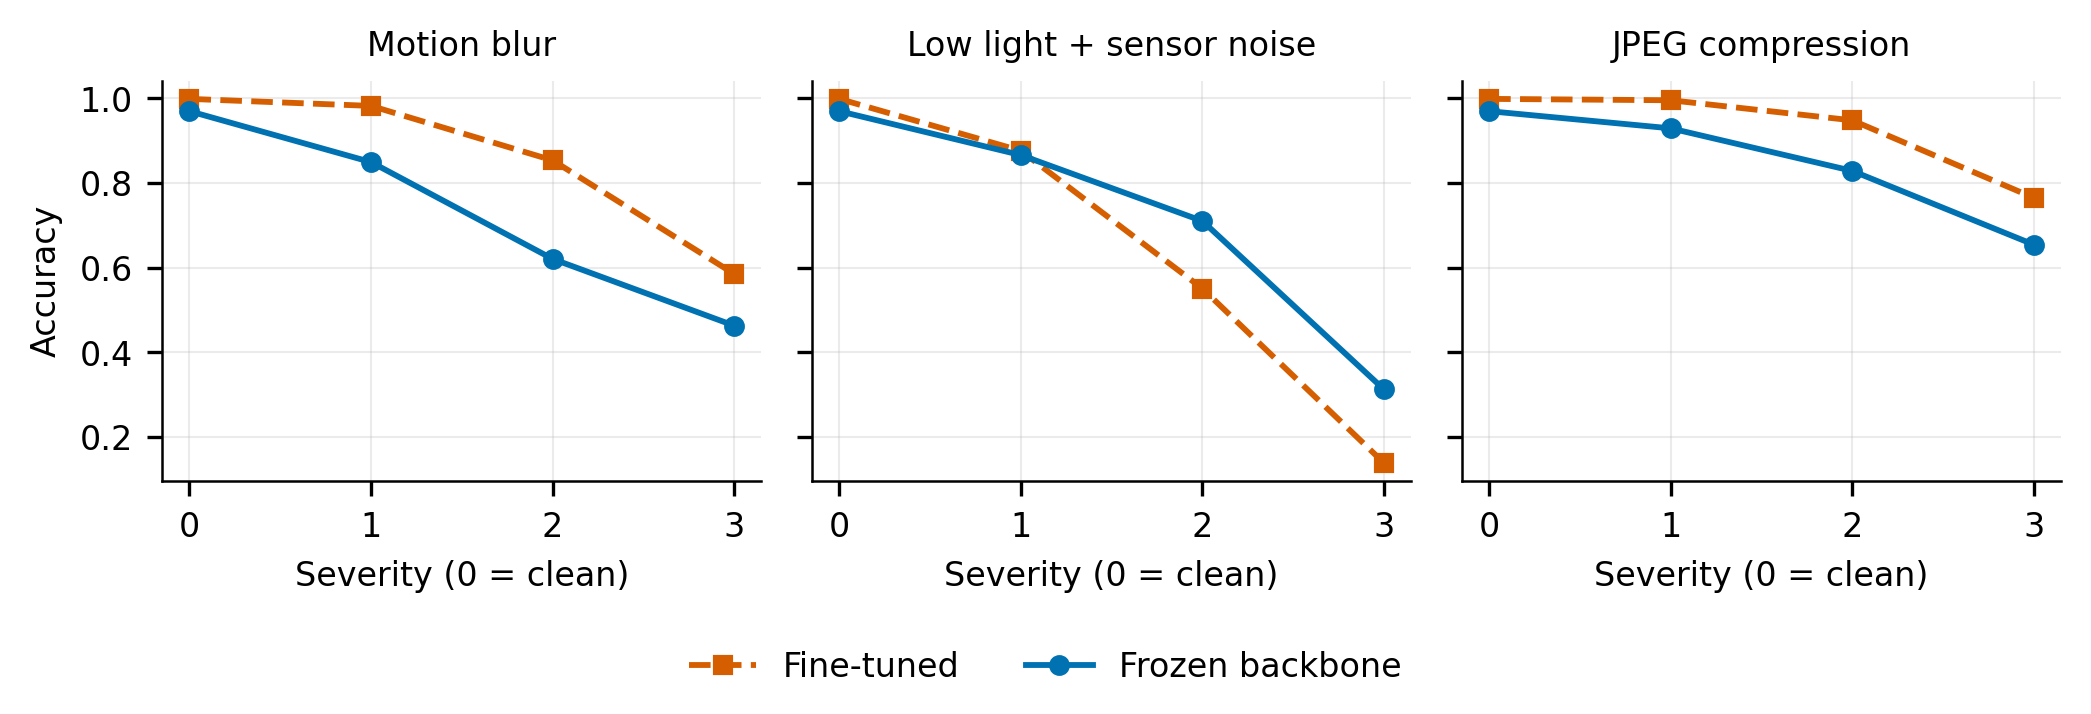
\includegraphics[width=0.93\textwidth]{degradation_accuracy.png}
\caption{Degradation under the three capture artifacts. Fine-tuning dominates under motion blur and
JPEG compression at every severity, but the curves cross between severity 1 and 2 under low light
with sensor noise, where the frozen backbone ends up 16 accuracy points ahead at severity 2.}
\label{fig:degradation}
\end{figure*}

Table~\ref{tab:clean} gives the clean comparison and Table~\ref{tab:robust} with
Figure~\ref{fig:degradation} the behaviour under degradation. The learning-rate ablation on the
fine-tuned condition gives 0.9986 / 0.9991 / 0.9963 accuracy for $10^{-4}$ / $10^{-3}$ / $10^{-2}$,
reaching the best epoch at 11 / 25 / 37 and costing 9.8 / 18.0 / 26.0 minutes. Because both
conditions share one ResNet-50 graph and the same parameter count, inference cost is a property of
the architecture and is measured once: 4.741\,ms per image at batch 1 (210.9\,img/s), 0.314\,ms at
batch 64 (3180.8\,img/s) and 773.1\,MB peak GPU memory on an A100.

\section{Interpretation}

On clean data fine-tuning is decisively better --- 3 errors against 66 --- and reaches its optimum in
a third of the epochs, because the frozen probe must solve a 38-way problem with 77\,862 parameters
on features never adapted to leaf texture. Under degradation the answer is conditional:
fine-tuning is markedly \emph{more} robust to motion blur and JPEG compression, by up to 23 accuracy
points, and \emph{less} robust to sensor noise from severity 2 onward. We read this as a
frequency-domain effect. Fine-tuning on noise-free laboratory images sharpens early filters onto
high-frequency texture statistics that only that capture regime produces. Blur and JPEG
\emph{remove or quantise} high-frequency content, leaving the adapted mid-level features to carry the
class signal, whereas sensor noise \emph{injects} random energy into exactly the band those filters
occupy. The frozen ImageNet backbone was trained on web photographs that already contain noise,
compression and uneven exposure, so it keeps a tolerance that fine-tuning trades away. The ablation
confirms the comparison is not an artefact of the learning rate: all three values land within 0.3
accuracy points of each other.

\section{Failure analysis}

\textbf{Clean data.} Every error of both models --- all 3 and all 66 --- is a confusion between two
diseases of the \emph{same crop}; the cross-crop error rate is exactly zero. The dominant pairs are
Corn Cercospora/Gray leaf spot $\rightarrow$ Northern Leaf Blight (2 of the 3 fine-tuned errors),
Tomato Bacterial spot $\rightarrow$ Late blight, Tomato Target Spot $\leftrightarrow$ Spider mites and
Tomato Early blight $\rightarrow$ Late blight. Inspection explains them: the fine-tuned model's corn
errors are leaves so far into necrosis that the lesion geometry separating the two diseases has been
consumed, and its tomato error is a leaf whose bacterial lesions have barely emerged. The visual
evidence for the true label is largely absent rather than ignored.

\textbf{Under degradation.} Fragility is class-dependent. At low light severity 2 the fine-tuned
model drops several classes from F1 near 1.0 to exactly 0 --- Potato healthy, Apple Cedar apple rust,
Raspberry healthy, Tomato Bacterial spot --- while the frozen model degrades the same classes
gracefully (Squash Powdery mildew $0.993 \rightarrow 0.259$ rather than to zero). The classes that
collapse first are those whose evidence is fine-grained: small specks and subtle colour shifts,
exactly what sensor noise masks. Healthy classes collapse because ``no lesion'' becomes
indistinguishable from ``lesion hidden by noise''.

\textbf{Calibration.} The fine-tuned model is badly calibrated when wrong: mean confidence on its
errors is 0.859 against 0.531 for the frozen model, and under motion blur severity 3 it still reports
0.858 while being right only 58.5\,\% of the time. For a deployed field system this is worse than the
accuracy it wins elsewhere, because the model does not signal that it has left its operating regime.

\textbf{Limitations.} Corruptions are simulated; a real robot would also introduce focus, perspective
and background variation. PlantVillage contains several images of the same physical leaf, so
clean-test accuracy overstates generalisation to new plants. Conclusions concern one architecture and
one dataset.

\section{Reproducibility}

Repository: \url{https://github.com/EgorSavchenko-web/icv2026-plant-disease}.
Environment: Python 3.12, torch 2.10.0, torchvision 0.25.0, CUDA 12.9, one NVIDIA A100 80\,GB PCIe
under a ClearML agent running the official CUDA 12.9.1 cuDNN runtime image on Ubuntu 24.04;
\texttt{requirements.txt} pins every dependency. Training takes 9.9 and 14.7 minutes; the robustness
sweep of 20 evaluation passes takes under two minutes. The test split is committed and both
checkpoints are published as release assets, so every reported number can be verified with
\texttt{5\_inference.py} and \texttt{6\_robustness\_eval.py} without retraining. Each run's ClearML
task id, worker, container, hyperparameters and timings are recorded in
\texttt{results/run\_provenance.json}, and corruptions are seeded per image, so they reproduce
byte-identically.

\section{Members' contributions}

\begin{tabular}{@{}p{2.3cm}p{5.6cm}@{}}
\toprule
\textbf{Member} & \textbf{Contribution} \\
\midrule
Egor\newline Savchenko & Research question and experimental design; system architecture; training,
inference, robustness and failure-analysis pipelines; verification and reproducibility. \\[3pt]
Zamir Safin & Dataset selection and provenance; split construction and leakage verification;
class-balance analysis; preprocessing and augmentation policy. \\[3pt]
Ilia\newline Ponomarev & Survey of existing plant-disease recognition solutions; backbone and
transfer-strategy selection; positioning of the results against published baselines. \\[3pt]
Vadim\newline Poponnikov & Technical summary, presentation slides and the live demo. \\
\bottomrule
\end{tabular}

\end{document}
